
\documentclass[11pt]{article}
\usepackage{geometry}                
\geometry{letterpaper}                   

\usepackage{graphicx}
\usepackage{amssymb}
\usepackage{epstopdf}

\usepackage[utf8]{inputenc}
\usepackage[english]{babel}
\usepackage{natbib}
\bibliographystyle{unsrtnat}
\renewcommand\bibsection{\section{\refname}}

\usepackage{amssymb, amsmath}
\usepackage[procnames]{listings}
\usepackage{color}
\usepackage[english]{varioref}
\usepackage{wrapfig}
\usepackage{pdfpages}

\DeclareGraphicsRule{.tif}{png}{.png}{`convert #1 `dirname #1`/`basename #1 .tif`.png}

\title{Vector based navigation of desert ants}
\author{Josua Graf, Noah Zarro}
\date{date} 

\graphicspath{ {./images/} }

\definecolor{keywords}{RGB}{255,0,90}
\definecolor{comments}{RGB}{0,0,113}
\definecolor{red}{RGB}{160,0,0}
\definecolor{green}{RGB}{0,150,0}
\lstset{language=Python, 
        basicstyle=\ttfamily\small, 
        keywordstyle=\color{keywords},
        commentstyle=\color{comments},
        stringstyle=\color{red},
        showstringspaces=false,
        identifierstyle=\color{green},
        procnamekeys={def,class}}

\begin{document}



\thispagestyle{empty}

\begin{center}
\includegraphics[width=5cm]{ETHlogo.eps}

\bigskip


\bigskip


\bigskip


\LARGE{ 	Lecture with Computer Exercises:\\ }
\LARGE{ Modelling and Simulating Social Systems\\}

\bigskip

\bigskip

\small{Project Report}\\

\bigskip

\bigskip

\bigskip

\bigskip


\begin{tabular}{|c|}
\hline
\\
\textbf{\LARGE{Vector based navigation of desert ants}}\\
\textbf{\LARGE{}}\\
\\
\hline
\end{tabular}
\bigskip

\bigskip

\bigskip

\LARGE{Josua Graf, Noah Zarro}



\bigskip

\bigskip

\bigskip

\bigskip

\bigskip

\bigskip

\bigskip

\bigskip

Zurich\\
\today
%Dec 2018\\

\end{center}



\newpage

%%%%%%%%%%%%%%%%%%%%%%%%%%%%%%%%%%%%%%%%%%%%%%%%%

\newpage
\section*{Agreement for free-download}
\bigskip


\bigskip


\large We hereby agree to make our source code for this project freely available for download from the web pages of COSS. Furthermore, we assure that all source code is written by ourselves and is not violating any copyright restrictions.

\begin{center}

\bigskip


\bigskip


\begin{tabular}{@{}p{3.3cm}@{}p{6cm}@{}@{}p{6cm}@{}}
\begin{minipage}{3cm}

\end{minipage}
&
\begin{minipage}{6cm}
\vspace{2mm} \large Josua Graf

 \vspace{\baselineskip}

\end{minipage}
&
\begin{minipage}{6cm}

\large Noah Zarro

\end{minipage}
\end{tabular}


\end{center}
\newpage

%%%%%%%%%%%%%%%%%%%%%%%%%%%%%%%%%%%%%%%



% IMPORTANT
% you MUST include the ETH declaration of originality here; it is available for download on the course website or at http://www.ethz.ch/faculty/exams/plagiarism/index_EN; it can be printed as pdf and should be filled out in handwriting



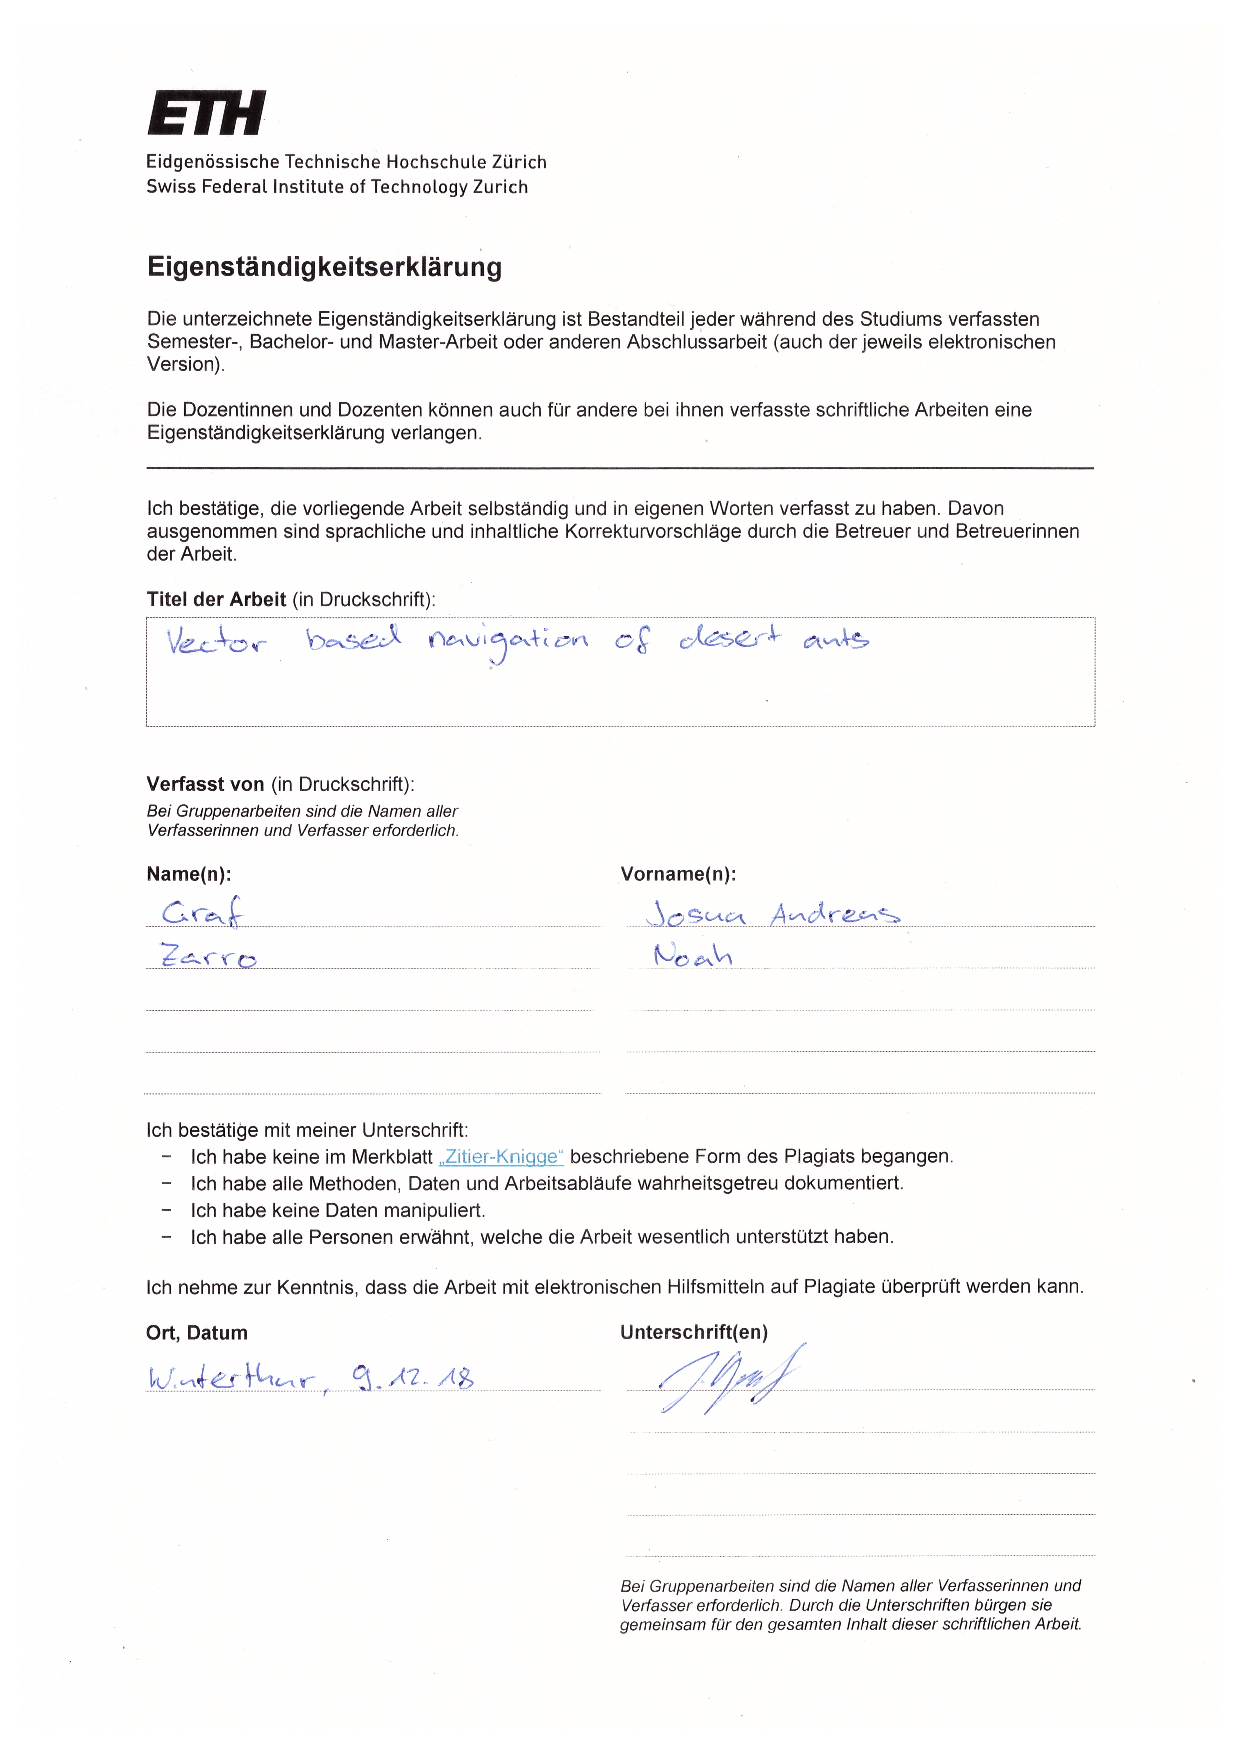
\includepdf[pages={1}]{formular.pdf}


%%%%%%%%%% Table of content %%%%%%%%%%%%%%%%%

\tableofcontents

\newpage

%%%%%%%%%%%%%%%%%%%%%%%%%%%%%%%%%%%%%%%



\section{Abstract} %Noah
	In this project we simulated the behavior of desert ants, as stated by R. S. Wehner in his report (\cite{wehner}). He conducted experiments with real ants and proposed a theory how these ants handle the orientation in the desert. We used his results to simulate an ant, which behaves as Wehner stated in his thesis and conducted his experiments again in simulation. It seams that our simulation matches the results of his real tests pretty well.
\newpage

\section{Individual contributions} %Noah
	N.Z and J.G set up a basic concept for the simulation, N.Z. and J.G. programmed the simulation, J.G. run the simulation, N.Z and J.G. wrote the report.
\section{Introduction and Motivations} %Josua
	\subsection{Motivation}
		Desert ants (\textit{Cataglyphis}) has a difficult task to navigate since there natural habitat has not much landmarks helping to find there way. Different scientific papers (\cite{mueller}), (\cite{wehner}), (\cite{knaden}) are postulating that desert ants use path integration as one component of there navigation. Because many technical applications are inspired by nature it is of high interest to have a clear idea how ants navigate in a unrecognizable landscape like desert. We could imagine a technical use in satellite steering or the navigation of evacuation robots in. 
	\subsection{Base Paper}
		This project is based on the paper "Local and global vectors in desert ant navigation" (\cite{wehner}). Through simulating an ant which follows the concepts of local and global vector described by \cite{wehner} and comparison with the actual behavior we wanted to find out if the concept postulated is complete or needs  adjustments. The goal was to implement the ant following the concepts as accurately as possible, then simulate the same test setup as it was used for the paper and compare the simulated plots with the plots from the experiments. 
	\subsection{Hypothesis}
		description of base paper (who did it, roughly what was it all about)
\section{Description of the Model} %Noah
	\subsection{Behavior of the ant}
		For our simulation we aimed to implement our model as closely as possible to the postulated model by Collett and his participants (\cite{wehner}). Their model splits the navigation of the ant in two parts. First, if there are no known landmarks in sight  (which is the usual case in the desert, the ants natural habitat) the ants orient themselves with a process named `path integration'. An ant leaving their nest to gather food counts each step it takes and measures its direction with aid of the sunlight, which it uses as a sort of compass. Like this it is always aware of its position relative to the nest and is able to find its way home. With this practice it is also less vulnerable to changes in the environment. The integrated value, respectively its negative which is pointing to the nest, is called the \texttt{global vector} by Collett and his colleagues. However, this practice becomes unreliable if the sun is not visible or the ant makes a mistake counting its steps. Therefore the ant also uses a different form of finding their way. It uses known landmarks, as for example rocks, bushes or other static objects for his orientation. Collett uses the word \texttt{local vector} to describe this form of orientation. Here it is important to say that as Collett says he does not calculate its \texttt{local vector} according to the direction of travel, like ''after the gray rock go left'', but relative to the cardinal direction, like ''after the gray rock go south''.
	\subsection{Conducted experiments}
	
\begin{wrapfigure}{r}{0.4\textwidth}
	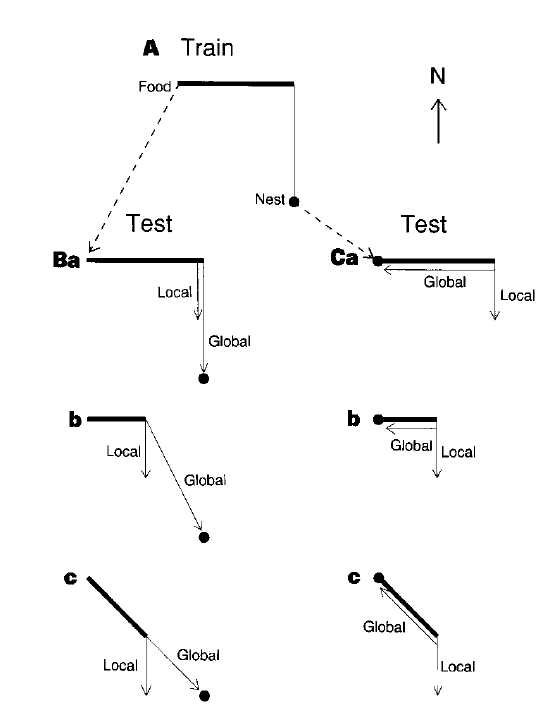
\includegraphics[width=0.4\textwidth]{experiments_setup.png}
	\caption{Test setup and some experiments conducted by Colletts. \cite{wehner}}
	\label{fig:setup}
\end{wrapfigure}

		To prove their theory the four researchers conducted several experiments. They built a training ground for the ants, where they had a nest, a feeding ground and a so called 'channel'. The channel was a tunnel dug in the ground just deeply enough that the ants could not see it form the surface. The ants were left in this training area, where they continuously gathered food and brought it back to the nest. So they got used to the setup and memorized the local landmarks and therefore set up their \texttt{local vector}. After a few days training the researchers started to conduct several different experiments, where they changed the setup partly. In some experiments they changed the the length and position of the channel, which disordered the ant's \texttt{local vector} and in some other cases they picked up the ant at their nest or on their way home and released it somewhere else, in order to give them a false estimation of their position according to the \texttt{global vector}, see~\vref{fig:setup}


\begin{wrapfigure}{l}{0.4\textwidth}
	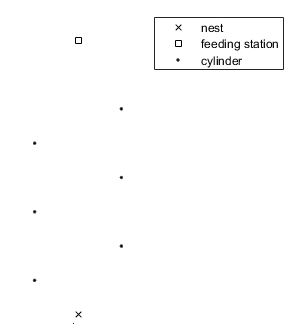
\includegraphics[width=0.4\textwidth]{cylinders.png}
	\caption{Training ground with cylinders.}
	\label{fig:cylinders}
\end{wrapfigure}


	Furthermore the group conducted an other kind of experiments, where they used no channel, but six highly visible black cylinders. They formed some kind of alley, where the ants had to get trough in order to reach their food. With this arrangement the ants were trained again, see~\vref{cylinders}. In the experiment conducted with those ants, they were picked up at the nest and released them at the feeding station.
		



\section{Implementation} % Noah
	\subsection{Main Concept}
		%we use an iterative approach, calculate local and global vector new in every step, merge them together(explain how). Save steps, plot them
		Our goal was to set up a simulation environment which was as general as possible, so we could easy switch between the test cases. The simulation is actually a huge loop, where in every iteration the ant does a step on a grid. It can just move horizontally, vertically and diagonal. This of course limits our ant, but if we simulate it with a big enough resolution it does not really matter. The ant can not reach every point on the map, there are several restrictions. First there is the channel, which can only be entered at specified channel exit or enter points. On the other hand the ant can not leave the map, so we constructed a virtual wall around the whole map, which it can not pass. Finally there is the nest, which we placed in the middle of the map.

In every iteration, the desired direction of the ant gets calculated according to the global and local vector in the \texttt{desired\_direction} function. Then we calculate all possible directions in the \texttt{possible\_direction} function. At the end the function \texttt{actual\_step} lets the ant walk one step and the global vector gets adjusted. If the ant did a certain amount of steps the simulation stops and the path gets plotted.

Our whole simulation environment is highly configurable, in the \texttt{conifg.py} file one can import any test file, in which all things like the map configuration, the start position of the ant etc. can be specified.
	\subsection{Global Vector}
		%explain how it gets calculated, and randomized
		The global vector starts with an initial value, which can be edited in the test file. In every iteration of the main loop the step conducted by the ant gets subtracted form the global vector. Additionally to model the imperfectness of the ants 0.1 mg brain we introduced two random factors. One gives credit to the fact, that a normal ant never walks in a straight line but rather zig-zags its way home. For this reason before a step is executed by the ant, the step gets randomly rotated, but with a gaussian distribution around the straight forward direction, see lst~\vref{lst:randomization}. The second randomization mirrors the fact that an ant never can memorize exactly how many millimeter it walked north or east. Thus the global vector gets slightly rotated randomly after every step, which means the ant does not exactly remember which way it took to get to its current position.
		
		
		
\begin{lstlisting}[caption={Randomization of desired step},label=lst:randomization]
# choose a random angle
sigma = con.sigma
randomAngle = np.random.normal(0, sigma)

# construct rotation matrix
rotationMatrix = [[math.cos(randomAngle), -math.sin(randomAngle)], [math.sin(randomAngle), 			   math.cos(randomAngle)]]

# rotate vector
rotated = np.matmul(rotationMatrix, desired)
\end{lstlisting}

	\subsection{Local Vector}
	%explain how it gets calculated and influenced by surroundings
		The local vector gets calculated every iteration and depends on the close surroundings of the ant. The influence and the position of these surroundings can be configured in the test files. The channel exit for example pushes the ant to the south. All these objects have a circular area of influence and the influence lowers quadratically with the ants distance to the object. All influences of all objects get summed up to the local vector and are merged with the global vector to the desired direction with the following formula:
		\begin{align*}
			desired\_direction = local\_vector * local\_weight + global\_vector * (1-local\_weight)
		\end{align*}
To calculate the local vector in the area of a familiar path the path is represented by a straight line with start and end point. Mathematically the straight is a linear function \( y(x)= m\times x + q \)and the vertical slope n is calculated by \( n = \frac {-1} {m}\) . 
\section{Simulation Results and Discussion}
	\subsection{Simulation Results} %Josua
		what did we get, is it the same
	\subsection{Discussion}
		what was different, probably the randomization was no as in real life
\section{Summary and Outlook} %Noah
	\subsection{Summary}
		it worked pretty well, Wehner did a good job, his experiments corresponds to our simulation, which was based on his theory. We do not know if its biologically correct
	\subsection{Outlook}
		we probably will not continue our research about desert ants, maybe Wehner will
\bibliography{bibliography}
\section{Latex-Stuff}

Beispielverweisung:

Hier wird auf dieses Bild verwiesen (fig.~\vref{fig:examplefigure})

Python Code:
\begin{lstlisting}[caption=Python code example]
import numpy as np

# show numbers 0-9
print ('Numbers from 0-9')
for i in range(10):
	print(i)
\end{lstlisting}


\begin{figure}[h!]
	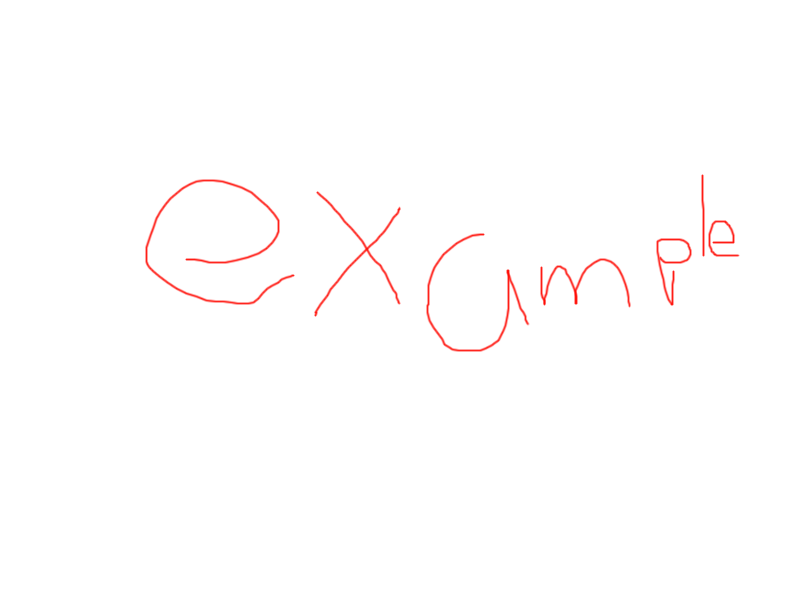
\includegraphics[width=0.5\textwidth]{example.png}
	\caption{Beispielbild, in Ordner images}
	\label{fig:examplefigure}
\end{figure}

Beispielliste:

\begin{itemize}
	\item erster Eintrag
	\item zweiter Eintrag
\end{itemize}



\end{document}  

\printbibliography

 
